
\begin{Exercise}[label={footfall_analysis}]
A concrete ribbed slab floor spans 9 m and has an average mass of \qty{500}{kg/m^2}. The floor is simply supported on either side and has a natural frequency of vibration of \qty{6.3}{Hz}. The floor is to be used for aerobics and other similar rhythmic activities at frequencies ranging from \qty{1.5}{Hz} to \qty{2.5}{Hz} and with contact ratios $\alpha$ between 0.5 and 1. During these activities the average imposed load will remain below \qty{0.75}{kN/m^2} (before dynamic magnification) and the damping ratio can be taken to be \qty{3}{\%}.

\begin{enumerate}[(a)]
    \item Determine the maximum possible resonant displacement and the resulting peak acceleration and bending moment per unit width.
    \item If the floor has been designed for a service load of \qty{5}{kN/m^2}, determine its suitability for the proposed use.
\end{enumerate}

\begin{center}
\pictures{beamPeople}
\hspace{1em}
\pictures{contactRatio}
\end{center}

\shortAnswer ...

References: \cite[page ??]{chopra}
\end{Exercise}



\begin{Answer}[ref={footfall_analysis}]
A transient walking force is a periodic loading with piecewise definition. Hence, two approaches may be followed. The first one consist on supperposing the solutions of the piecewise excitating force. The solution will be analytical, but according to a piecewise definition. The second approach is more generic, it consist on approximating the pulse by a Fourier series. There will be a truncation error, but the procedure is valid for any arbitrary pulse. In this exercise we will follow the Fourier series approach.



\paragraph{Pre computed Fourier terms}
Each component of a Fourier series is also known as harmonic. For a half sine activity, the amplitude of the first harmonics is

\begin{center}
\begin{tabular}{|l|c|cccc|}
    \hline
    Activity & $\alpha$ & $F_1/mg$ & $F_2/mg$ & $F_3/mg$ & $F_4/mg$ \\ \hline
    Walking  &    2/3   &   1.29   &   0.16   &   0.13   &   0.04   \\
    Exercise &    1/2   &   1.57   &   0.67   &   0.00   &   0.13   \\
    Jumping  &    1/3   &   1.80   &   1.29   &   0.67   &   0.16   \\
    High jumping & 1/4  &   1.89   &   1.57   &   1.13   &   0.67   \\ \hline
\end{tabular}
\end{center}


\paragraph{Calculation of the Fourier terms}
Most commonly, Fourier series are expressed as a linear combination of $\sin$ and $\cos$,
$$
F(t) \approx \frac{a_0}{2} + \sum_{n=0}^{\infty} \left(a_n\cos(n\Omega t) + b_n\sin(n\Omega t)\right)
$$
with
\begin{align*}
a_0 &= \frac{2}{T}\int_{0}^{T} F(t) dt \\
a_n &= \frac{2}{T}\int_{0}^{T} F(t) \cos(n\Omega t) dt \\
b_n &= \frac{2}{T}\int_{0}^{T} F(t) \sin(n\Omega t) dt \\
\end{align*}

An alternative form is to compute the combination of the trigonometric functions as
$$
F(t) \approx F_0 + \sum_{n=0}^{\infty} F_n\sin(n\Omega t + \phi_n)
$$
with
\begin{align*}
&F_0 = \frac{a_0}{2} \\
&F_n = \sqrt{a_n^2 + b_n^2} \\
&\tan\phi_n = \frac{b_n}{a_n} \\
\end{align*}


\begin{center}
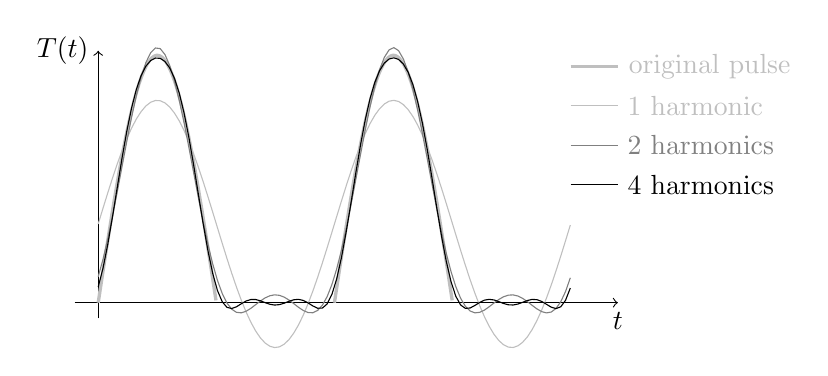
\begin{tikzpicture}[domain=0:2, xscale=3, samples=100]
    \draw[->] (-0.1,0) -- (2.2,0) node[below] {$t$};
    \draw[->] (0,-0.2) -- (0,3.2) node[left] {$T(t)$};

    % \x r means to convert '\x' from degrees to radians:
    \draw[very thick,lightgray,domain=0:0.5] plot (\x,{pi*sin(2*pi*\x r)});
    \draw[very thick,lightgray,domain=1:1.5] plot (\x,{pi*sin(2*pi*\x r)});
    \draw[lightgray] plot (\x,{1+1.57*sin(2*pi*\x r)});
    \draw[gray] plot (\x,{1+1.57*sin(2*pi*\x r)-0.67*cos(4*pi*\x r)});
    \draw[black] plot (\x,{1+1.57*sin(2*pi*\x r)-0.67*cos(4*pi*\x r)-0.13*cos(8*pi*\x r)});

    \draw[very thick,lightgray] (2,3)   -- +(.2,0) node[right] {original pulse};
    \draw[lightgray]            (2,2.5) -- +(.2,0) node[right] {1 harmonic};
    \draw[gray]                 (2,2)   -- +(.2,0) node[right] {2 harmonics};
    \draw[black]                (2,1.5) -- +(.2,0) node[right] {4 harmonics};
\end{tikzpicture}
\end{center}

\end{Answer}
